\begin{figure*}[!t]
    \centering
    \hspace*{-5mm}\subfigure[MI Convergence]{
      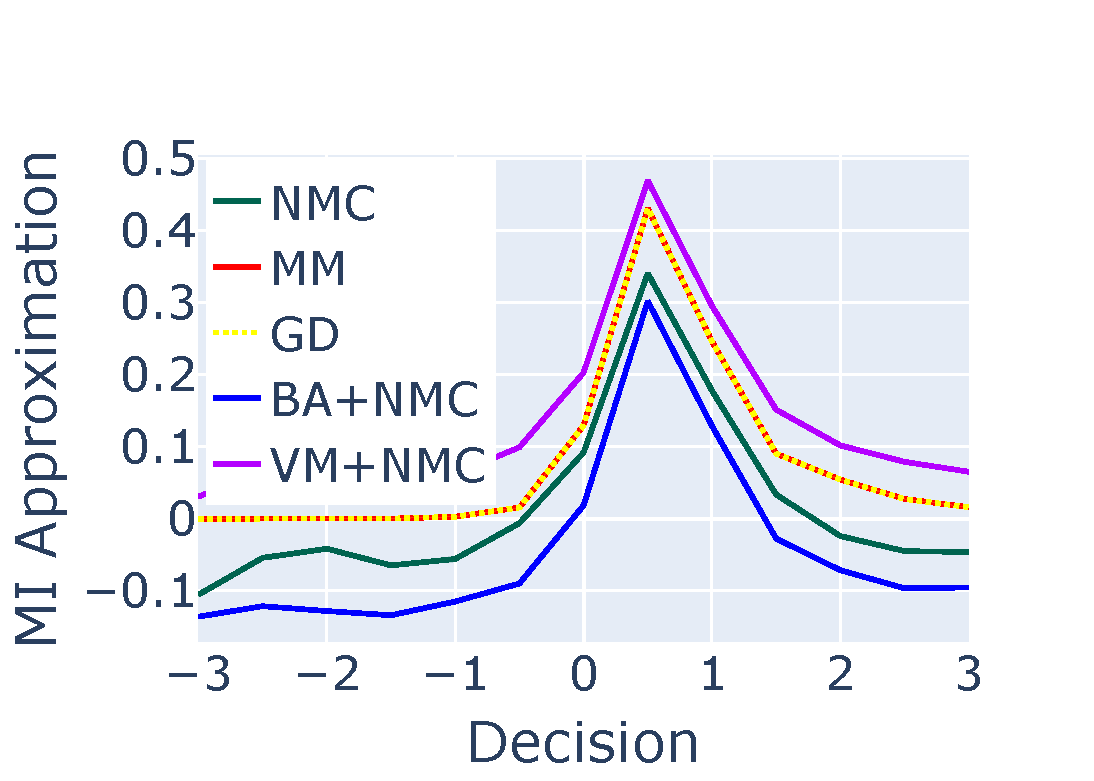
\includegraphics[width=.36\textwidth]{ExtrapolationMI.pdf}
    }
    \hspace*{-7mm}\subfigure[Computation Time]{
      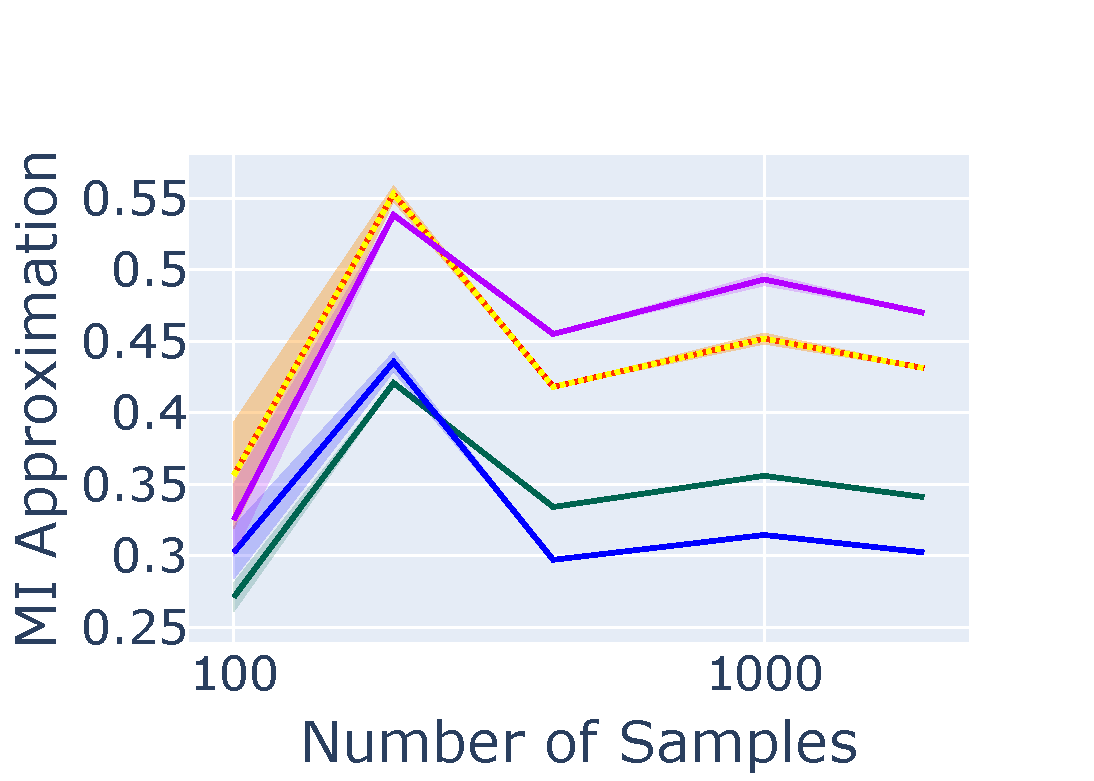
\includegraphics[width=.36\textwidth]{ExtrapolationConverge.pdf}
    }
    \hspace*{-7mm}\subfigure[Samples]{
      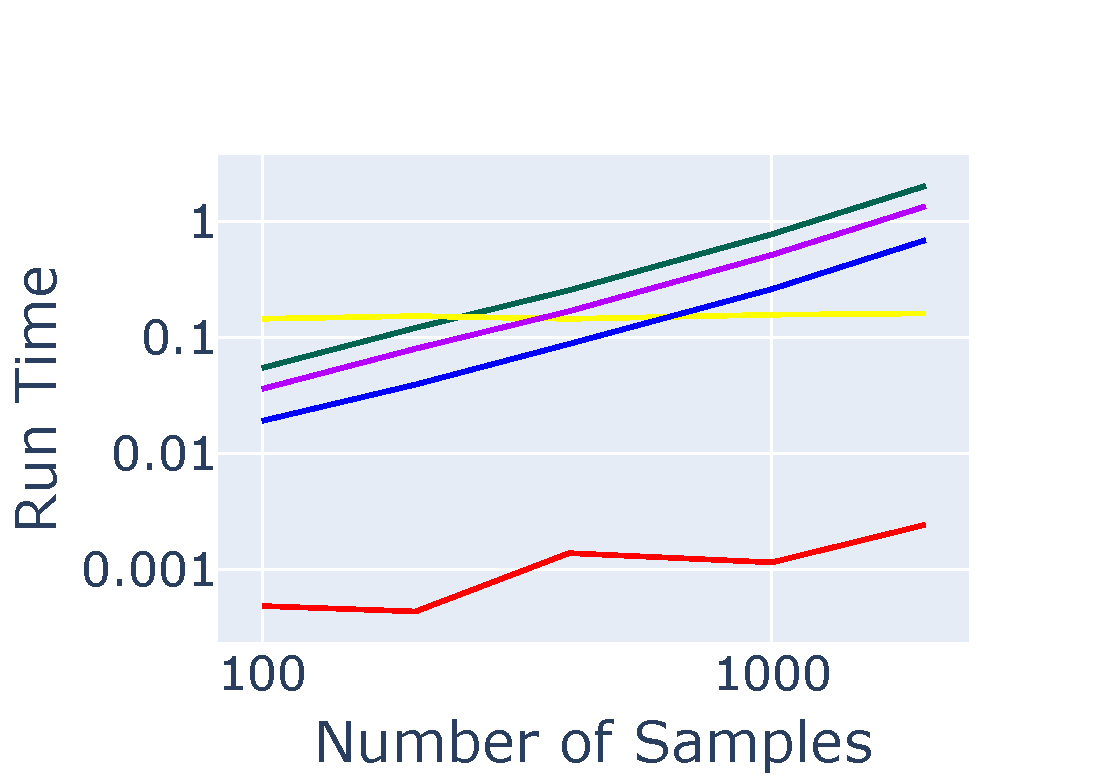
\includegraphics[width=.36\textwidth]{ExtrapolationTime.pdf}
    }
    \caption{\small \textbf{Extrapolation} (a) The MI for decisions $d
      \in [-3,3]$ with variances $\sigma_x^2 = 3$, and $\sigma_y^2=1$
      for each approximation with 4000 samples is plotted with $d=.5$
      being the maximum. Note the negative bias resulting from
      NMC. (b) The convergence rate versus samples is plotted at
      maximum decision ($d=.5$) (c) The run time for each method is
      plotted with moment matching being orders of magnitude faster than
      any other method.}
    \label{fig:Extrapolation}
\end{figure*}

We adapt the following experiment from Foster et
al.~(\citeyear{Foster2019}) intended to evaluate the implicit
likelihood MI estimator $\Iml$ (or $\hat{I}_{m+\ell}$).  Labeled
information, $y$, from a subset of the design space is be used to
predict labels at a location $x$ that can't be directly observed. The
model is as follows,
\[
 \psi\sim \Ncal(\mu_\psi, \Sigma_\psi), \quad  \theta \mid \psi \sim \Ncal\left( (X_\theta^T \psi)^2, \sigma_x^2 \right) \quad y\mid\psi,d \sim \Ncal\left( (X_d^T \psi)^2, \sigma_y^2 \right)
\]
where $X_x = (1,-\frac{1}{2})$ and $X_d = (-1,d)$.  The aim is to
choose a design $d \in \mathbb{R}$ that maximizes $I(\theta ; Y \mid
d)$.  Thus, $\psi$ is a nuisance variable that must be marginalized.
This marginalization lacks a closed-form and so the likelihood $p(y
\mid \theta)$ is implicit--it cannot be evaluated nor efficiently
sampled.  As a baseline we draw $N$ samples from the joint and use the
NMC estimator to compute entropies as:
\begin{equation}
    H(\theta)= -\int p(\theta)\log(p(\theta))dx \approx -\dfrac{1}{N}\sum_i \log\left(\dfrac{1}{N-1}\sum_{j\neq i}p(\theta_i|\psi_j)\right)
    \label{eq:NMCentropy}
\end{equation}
%% To compute each of these methods, we will sample from $x_i,y_i,\psi_i
%% \sim p(\psi)p(x|\psi)p(y|\psi,y)$ and we will need to compute a NMC
%% estimator for the $H_p(p)$ terms in $\Imarg$ and $\Ipost$ as well as
%% for a total approximation of $I(X,Y)\approx I_{NMC}(X,Y)$. To compute
%% each entropy term from samples, we use

\FIG\ref{fig:Extrapolation} summarizes the proposed estimators and
runtime.  As the theory suggests our moment matching estimators
provide substantial speedup, and we observe accurate estimates with
$\Iml$ in this model.  We emphasize that $\Imarg$ and $\Ipost$ are
infeasible due to the need to estimate model entropies in this
implicit likelihood model.  We instead augment these methods with the
NMC estimator (e.g. \EQN\eqref{eq:NMCentropy}), which is referred to
as \emph{variational NMC} in the literature~\cite{Foster2019}.
However, the finite sample bias of NMC violates expected bound
properties for few samples--see \FIG\ref{fig:Extrapolation} (center).
We include these estimators to highlight the difficulty of estimating
MI in implicit likelihood models and to emphasize their practical
limitations.

%% An issue with this approximation is that despite it being consisent, it is biased
%% and the bias decays slowly (Zheng, 2018). When we observe Figure
%% ~\ref{fig:Extrapolation}(a)(b), we notice that the NMC is negative for some 
%% values of $d$. $I(X,Y)\geq0$ so this is the effect of the bias. Likewise, since 
%% the Variational Posterior and Variatoinal Marginal use entropy terms computed
%% using the NMC, they too are biased. However, we do notice that we maintain the 
%% ordering of the approximators from Lemma~\ref{lemma:MIOrder}.\\
%% From the experiment, we see that the optimal decision is when $d=.5$. This makes
%% intuitive sense for our problem as $X_x=(1,-\frac{1}{2})$ and 
%% $X_d = (-1,\frac{1}{2})$ which implies that they are highley negatively 
%% correlated, giving infromation about one another. As for the run time in (c), we
%% notice that Moment Matching is uniformaly faster than any other method by a few
%% orders of magnitude. Also, after approximatley 500 samples, the gradient decsent
%% based method becomes computationally cheaper than the NMC methods.\\
%% From this experiment, we see that moment matching provides a qualitatively good 
%% estimation as any other method while simulateously saving orders of magnitude in
%% computation time.\\
